% Q29. Tengo acceso a materiales de apoyo para usar chatbots en el estudio de matemáticas (tutoriales, guías, etc.)
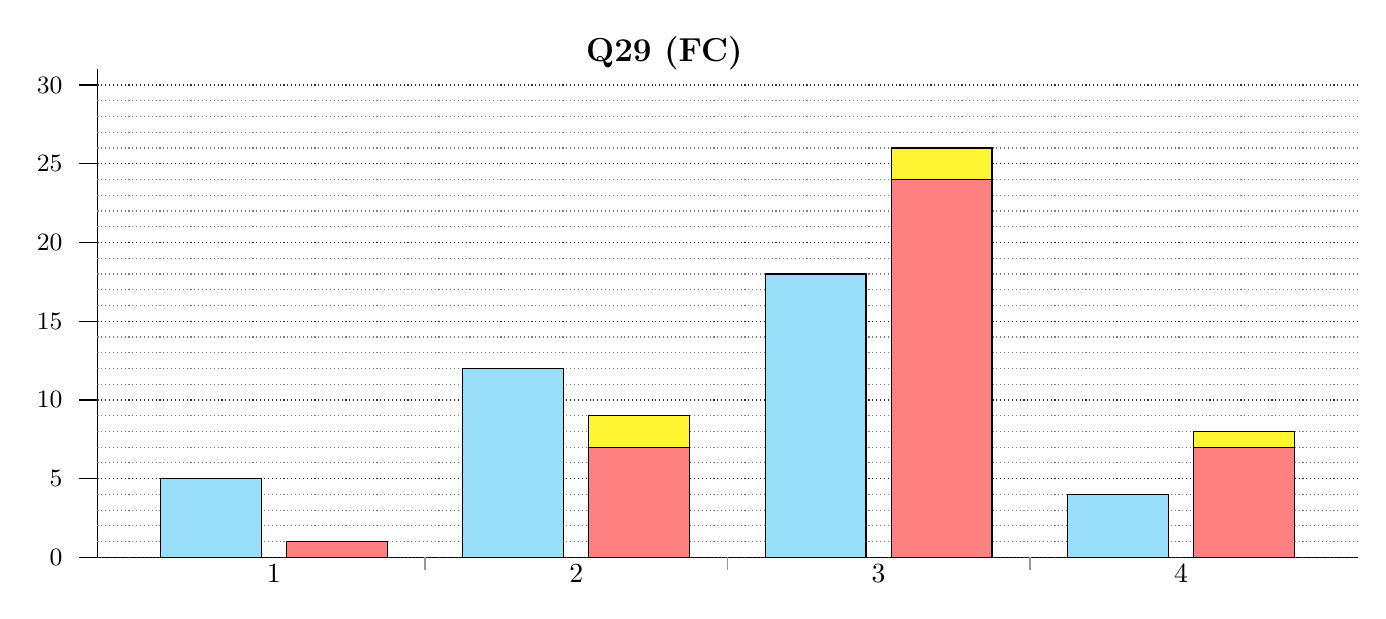
\begin{tikzpicture}[y=0.2cm, x=1.6cm]
  % Ejes
  \draw (0,0) -- (10,0);
  \draw (0,0) -- (0,31);

  % Cuadrícula cada 5 (más oscura) con números
  \foreach \y in {0,5,...,30} {
    \draw[densely dotted,black!80] (0,\y) -- (10,\y);
    \draw (-0.15,\y) -- (0,\y);
    \node[left] at (-0.2,\y) {\small \y};
  }
  
  % Cuadrícula cada 1 (más clara) sin números
  \foreach \y in {1,2,3,4,6,7,8,9,11,12,13,14,16,17,18,19,21,22,23,24,26,27,28,29} {
    \draw[densely dotted,black!50] (0,\y) -- (10,\y);
  }

% Marcas divisorias (centradas)
\foreach \x in {2.6,5.0,7.4} {
  \draw[gray!80,line width=0.6pt] (\x,-0.8) -- (\x,0);
}

  % Etiquetas eje X (centradas en cada grupo)
  \node at (1.4, -1) {1};
  \node at (3.8, -1) {2};
  \node at (6.2, -1) {3};
  \node at (8.6, -1) {4};

  % PRE (azul)
  \fill[cyan!40,draw=black] (0.5,0) rectangle (1.3,5);
  \fill[cyan!40,draw=black] (2.9,0) rectangle (3.7,12);
  \fill[cyan!40,draw=black] (5.3,0) rectangle (6.1,18);
  \fill[cyan!40,draw=black] (7.7,0) rectangle (8.5,4);

  % POST (rojo + amarillo)
  % Cat 1
  \fill[red!50,draw=black]    (1.5,0) rectangle (2.3,1);

  % Cat 2
  \fill[red!50,draw=black]    (3.9,0) rectangle (4.7,7);
  \fill[yellow!80,draw=black] (3.9,7) rectangle (4.7,9);

  % Cat 3
  \fill[red!50,draw=black]    (6.3,0) rectangle (7.1,24);
  \fill[yellow!80,draw=black] (6.3,24) rectangle (7.1,26);

  % Cat 4
  \fill[red!50,draw=black]    (8.7,0) rectangle (9.5,7);
  \fill[yellow!80,draw=black] (8.7,7) rectangle (9.5,8);

  % Título
  \node[font=\bfseries\large] at (4.5,32) {Q29 (FC)};
\end{tikzpicture}